\section{YOLOv1}  \label{sec:yolov1}

The first YOLO model was proposed in the "You Only Look Once: Unified, Real-Time Object Detection" paper in 2015 \cite{yolov1_2016}. Since there will be improvement version of the model, we denote this first model is YOLOv1, which is widely accepted in the computer vision research community \cite{understand_cnn_vs_yolo}. The YOLOv1 is designed to be a realtime object detection model. The YOLOv1 model is a three steps process, as shown in Firgure \ref{fig:yolov1_process}. In the first step, the model take an image of any size as input and resize the image to the fix size of $448 \times 448$. In the second step, the model predict mutiple bounding box, each with a objectiveness confidence score, and multiple classification for each detected object. Since the model predict multiple bounding box and classfication for each detected object, a non-maximum suppression (NMS) algorithm, as described in Subsection \ref{subsec:rpn}, is applied to assign one bounding box and one classification label per predicted object in the last step.

\begin{figure}[!ht]
    \centering
    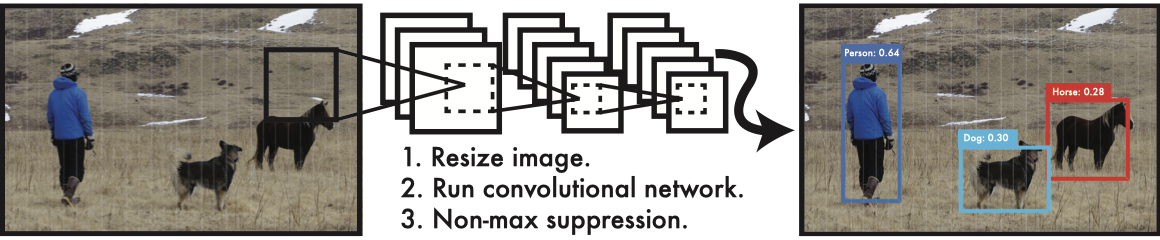
\includegraphics[width=4in]{figures/yolov1_process.png}
    \caption{YOLOv1 object detection process \cite{yolov1_2016}} 
    \label{fig:yolov1_process}
\end{figure}

In the original paper, the authors claim that YOLOv1 model have three main benifit \cite{yolov1_2016}. First, YOLOv1 is extremely fast, processing 45 images per second compare to 7 images per second achieved by the Faster R-CNN model with VGG16 backbone. However, this is achieved at the cost of 9.8\% reduction in mean average precision (mAP) score, i.e., 63.4\% and 73.2\% for mAP score of YOLOv1 and Faster R-CNN, respectively. The second benifit is YOLOv1 learn a general representation of object, thus it tend to perform better compare to R-CNN based model when predicting for other domain like artwork. The third benifit it it see the entire image during bounding box regression and classification compare to R-CNN classifier and bounding box regressor only see the ROI. This change allow YOLOv1 to encodes contextual information about classes and thus reduce the number of false positive.

\subsection{Network Architecture}

\begin{figure}[!ht]
    \centering
    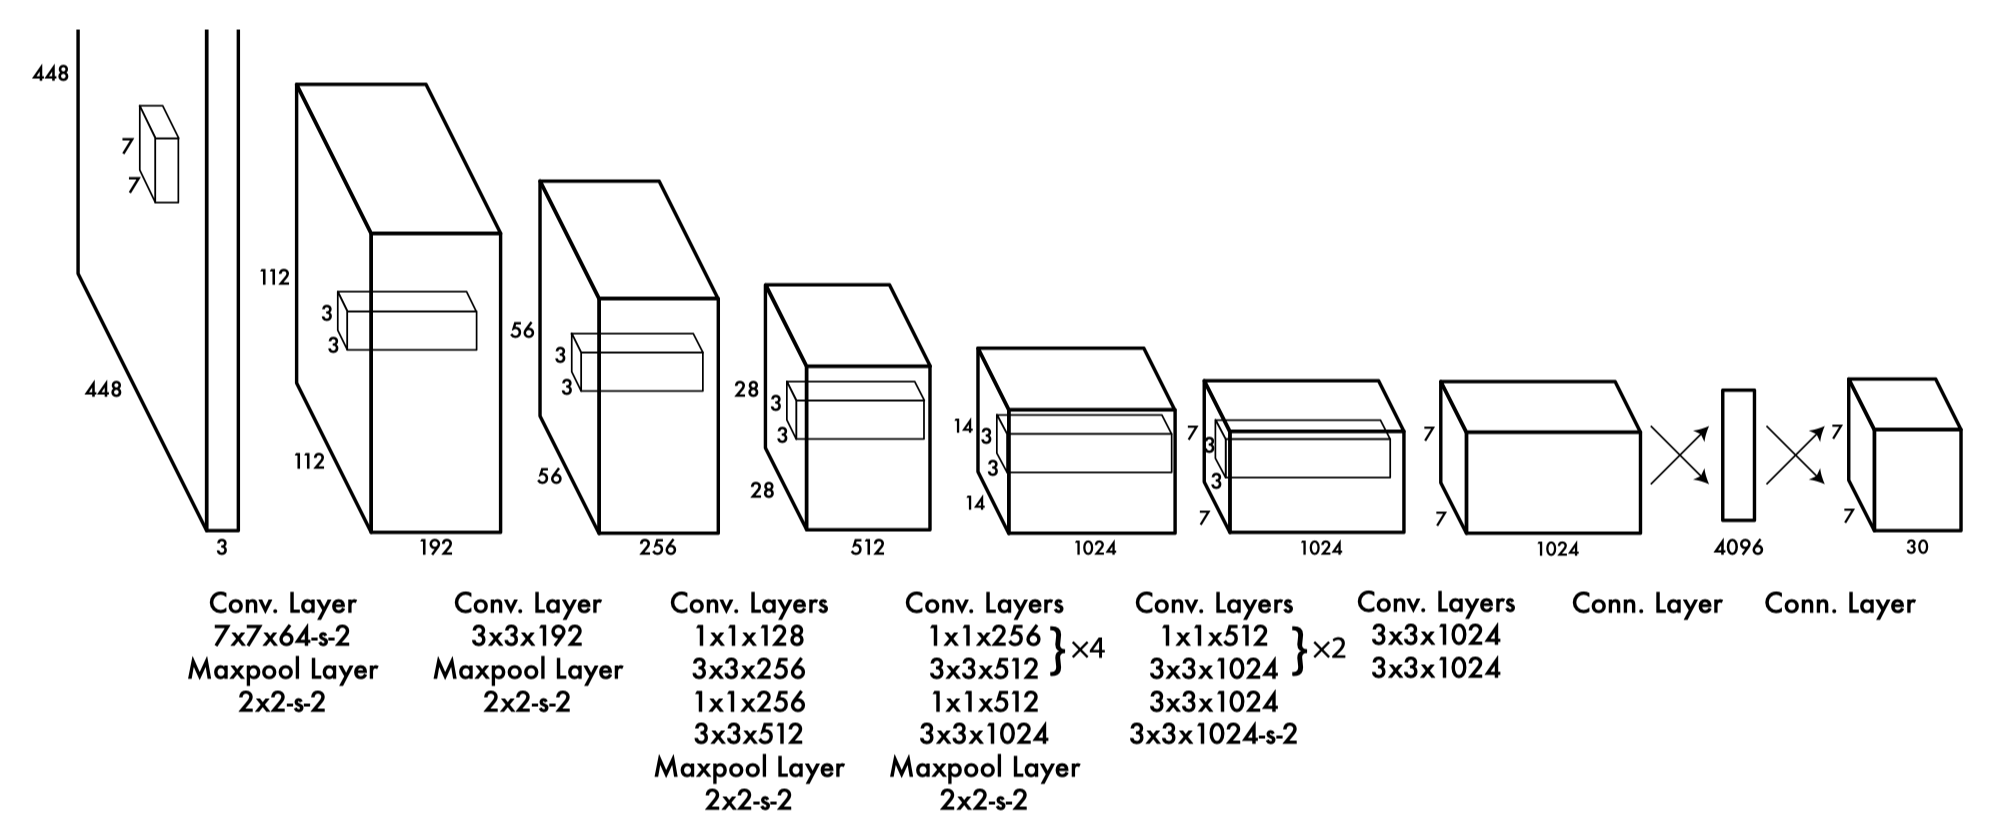
\includegraphics[width=4in]{figures/yolov1_archite.png}
    \caption{YOLOv1 architecture \cite{yolov1_2016}} 
    \label{fig:yolov1_archite}
\end{figure}

The YOLOv1 model is a convolutional neural network (CNN) based on the GoogLeNet model for image classification {\color{red} cite GoogLeNet}. The YOLOv1 model consist of 24 convolutional layer and end with 2 fully connected layer. The overall architecture of YOLOv1 netword is shown in Figure \ref{fig:yolov1_archite}. The author replace the inception layers in GoogLeNet with $1 \times 1$ reduction layer and $3 \times 3$ convolutional layer pair {\color{red} further explain the inception modules and reduction layer}. All the layers in the yolov1 network, with the exception of the final layer, utilize the leaky ReLU activation function {\color{red} cite leaky ReLU}, described as:
\begin{equation*}
    \phi(x) = {\color{red}x if x > 0, 0.1 x otherwise}
\end{equation*}

As we can see in Figure \ref{fig:yolov1_archite}, the last convolutional layers in the network produce a feature map of size $7 \times 7 \times 1024$. This feature map is then processed by two fully connected layers. The last fully connected layer is responsible for predicts both the bounding box and the class label probability \cite{yolov1_2016}. This layer use a linear activation function. The classfication process in the last fully connected layer is simmilar to other CNN where the layer is randomly initialize and can be optimized through training. On the other hand, YOLOv1 proposed a new bounding box regression method that able to  predict all bounding box of all objects present in the image at once, instead of processing each RoI individually one-by-one like the regressor implemented in Faster R-CNN. We will discuss this bouding box generation process in the next subsection.

\subsection{Bounding Box Generation}
To predict bounding box, the YOLOv1 model divide the image into an $S \times S$ grid of equal cells. Each grid cell is then predict $B$ bounding boxes and $C$ probabilities for the $C$ supported classes \cite{yolov1_2016}. The $S$ and $B$ values are hyperparameter and can be fine tune throught experiment. The $C$ value is the number of classes in the training dataset. In other words, $C=20$ if the training dataset is PASCAL VOC \cite{pascal_voc_2015} and $C=80$ if the training dataset is COCO dataset \cite{coco_2014}.

Each bounding box is represented by 5 values: coordinate $x$, coordinate $y$, width $w$, height $h$, and a confidence score. The $(x, y)$ coordinates is the center of the bounding box relative to a grid cell. The width $w$ and height $h$  is the dimension of bouding box in 2D space. The value of $w$ and $h$ are normalized with respect to the input image width and height, thus they are bounded by [0, 1]. The confidence score denote the model confidence in saying there is an object present in this cell, i.e., the objectiveness probability.

\begin{figure}[!ht]
    \centering
    \subfloat[][{\color{red} tobe added}]{ 
        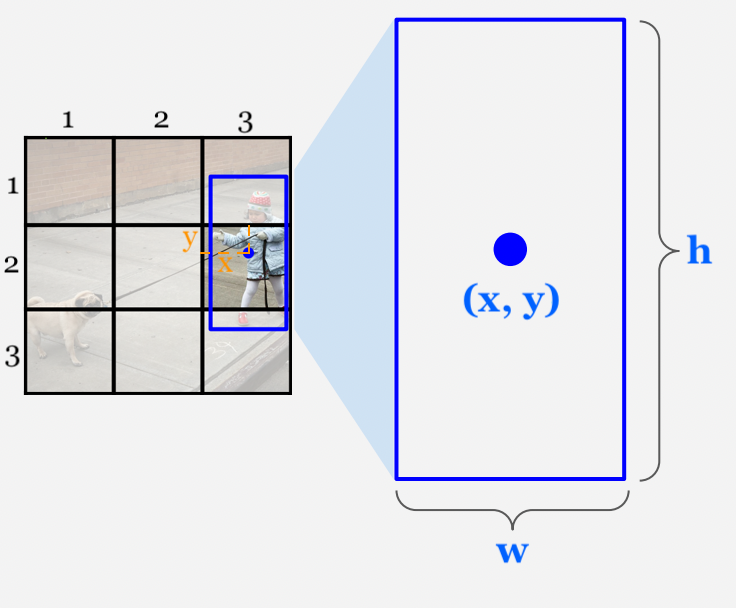
\includegraphics[height=2in]{figures/yolov1_bbox1.png} \label{fig:yolov1_bbox1}
    }
    \qquad \qquad
    \subfloat[][{\color{red} tobe added}]{ 
        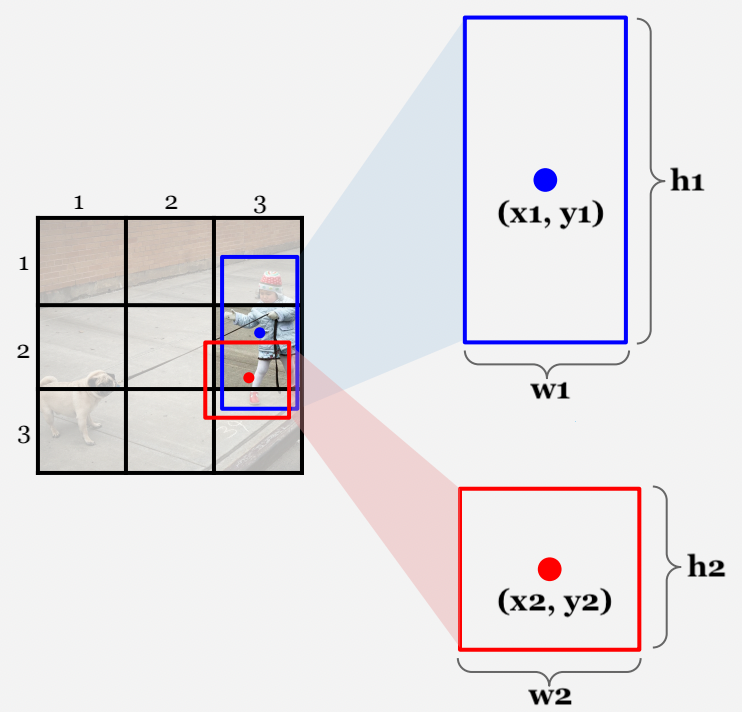
\includegraphics[height=2in]{figures/yolov1_bbox2.png} \label{fig:yolov1_bbox2}
    }
    \caption{{\color{red} tobe added}}
\end{figure}

As an example, consider processing an image with $S=3$, $B=1$, and clasifying between two class human and dog ($C=2$), as demonstrated in Firgure \ref{fig:yolov1_bbox1}. Since $B=1$, which means we only predict one bounding box per cell, then the cell$_{32}$ will return a tensor represent the predicted bounding box as:
\begin{equation*}
    ceil's\ output = \begin{bmatrix}
        {\color{blue} x \quad y \quad w \quad h \quad conf} \quad p_{human} \quad p_{dog}
        \end{bmatrix}
\end{equation*}
where $conf$ is the confidence score, $p_{human}$ and $p_{dog}$ are probability that the object belong to the human and dog class, respectively. Noted that when we only predicting 1 bounding box per ceil, the YOLOv1 model predict $(4+1+2)$ values for each ceil, where 4 value describe the bounding box location, 1 for confidence score, and 2 probality values with one for each class. Therefore we say that when $B=1$, the model predict $(4+1+C)$ for each ceil. 

Now, we consider the example reside in Figure \ref{fig:yolov1_bbox2}, which is the same setup as previous example but with $B=2$. In this second example, we predict two bounding boxes per cell, then the cell$_{32}$ return the following tensor for the two bounding boxes:
\begin{equation*}
    ceil's\ output = \begin{bmatrix}
        {\color{blue} x_1 \quad y_1 \quad w_1 \quad h_1 \quad conf_1} \quad 
        {\color{red} x_2 \quad y_2 \quad w_2 \quad h_2 \quad conf_2} \quad 
        p_{human} \quad p_{dog} 
    \end{bmatrix}
\end{equation*}
The ceil output a $(4+1)*2+C$ elements tensor for when the model predict two bounding boxes per ceil. Therefore, we can generalize the ceil's prediction is encoded as $(4+1)*B+C$ tensor.

The computed prediction for each ceil in the grid is stacked side by side create the depth for the image. That is we divides a 2-dimentional image into a grid of $S \times S$ ceil, we predict a $(4+1)*B+C$ tensor for each ceil, these prediction create the third dimention of the image. Therefore the prediction for the image is encoded as $S \times S \times [(4+1)*B+C]$ tensor. 

The YOLOv1 architecture showned in Figure \ref{fig:yolov1_archite} is for predicting 20 class in PASCAL VOC with $S=7$ and $B=2$, thus the model predicting a $7 \times 7 \times 30$ tensor which encoded multiple bouding boxes and classfication for each ground-truth object. 

\subsection{Training}
The first 20 convolutional layers of YOLOv1 is pretrained with the input size of $224 \times 224$ for classification task on the ImageNet2012 dataset \cite{ImageNet_dataset}. Then four new convolutional layers and 2 fully connected layer are added. These new layers are randomly initialize. Additionally, the input size is increase to $448 \times 448$ for object detection task \cite{yolov1_2016}. With the initialized network, the model generate multiple bounding boxes and classification as described previously. While the YOLOv1 model apply NMS to choose which predicted bounding box to keep at inference time, the author used a different scheme to choose which predicted bounding box to contribute to the loss function. The scheme is choosing the predictor with predicted box that has the highest IoU with a ground truth box. This lead to each predictor have different specilization, which mean each predictor is better at predicting certain size, aspect ratio, or object's class \cite{yolov1_2016}.

The YOLOv1 model is trained to optimize for the sum-square error which encode both the bounding box coordinate loss and the classification loss \cite{yolov1_2016}. While sum-square error allow eazier optimization, it have some shortcomming and not ideal if the model need to optimize for average precision. The first critical shortcomming is the loss weight localization error and classification error equally \cite{yolov1_2016}. In an image, since the majority of the cells does not contain any object, which mean confidence score for these cell are 0, thus cause model always have a poor performance for classification task. This also cause bouding box error to have little affet on the total error. Thus a scalar term is added to the loss to weight the bouding box error higher than the classification error \cite{yolov1_2016}. The second critical shortcomming is sum-squared error weight offset in large bounding box and small bounding box equally \cite{yolov1_2016}. This is not ideal as offset by certain pixels have a larger affect on the smaller bouding box than the larger bounding box, due to total number of pixels in large bounding box is larger than the smaller bounding box. To patially resolve this, the YOLOv1 model perform the error calculation on the squareroot of bounding box width and height instead of the width and height directly.